% !TeX root = ../main.tex
\chapter{绪论}
\label{chap:introduction}

本章用于展示正文一级标题、二级标题、三级标题、文献引用和图环境的写法。正式写作时，应将本章替换为研究背景、国内外研究现状、研究问题、研究内容和论文结构安排等内容。章节编号由 \LaTeX{} 自动生成，正文引用章节时使用 \verb|\label| 与 \verb|\ref|，例如第~\ref{chap:method-example} 章展示方法与公式写法。

本模板由马千里整理，贡献者 GitHub 信息见脚注\footnote{\href{https://github.com/Yuki-zik}{GitHub: Yuki-zik}}。本句也示范了在脚注中使用超链接的写法，正式论文中可按需删除或替换为论文相关注释。

\section{研究背景与意义}
\label{sec:background}

正文默认使用中文宋体小四、英文 Times New Roman、1.5 倍行距、首行缩进 2 字符。引用文献时使用 \verb|\cite{key}|，例如视觉语言模型研究可写作 \cite{sample-vlm}，模型审计或方法类文献可写作 \cite{sample-method}。正式论文中，事实性判断、方法来源和对比对象均应给出可靠引用。

\section{国内外研究现状}
\label{sec:related-work}

图题格式由模板自动设置为“图章号-图号  图题”。正文引用图时使用“图~\ref{fig:ningbo-university-gate}”。图~\ref{fig:ningbo-university-gate} 使用一张真实图片作为插图示例；正式论文中，应替换为与正文内容直接相关的自有图片、实验图或已获授权的公开图片。

\begin{figure}[htbp]
  \centering
  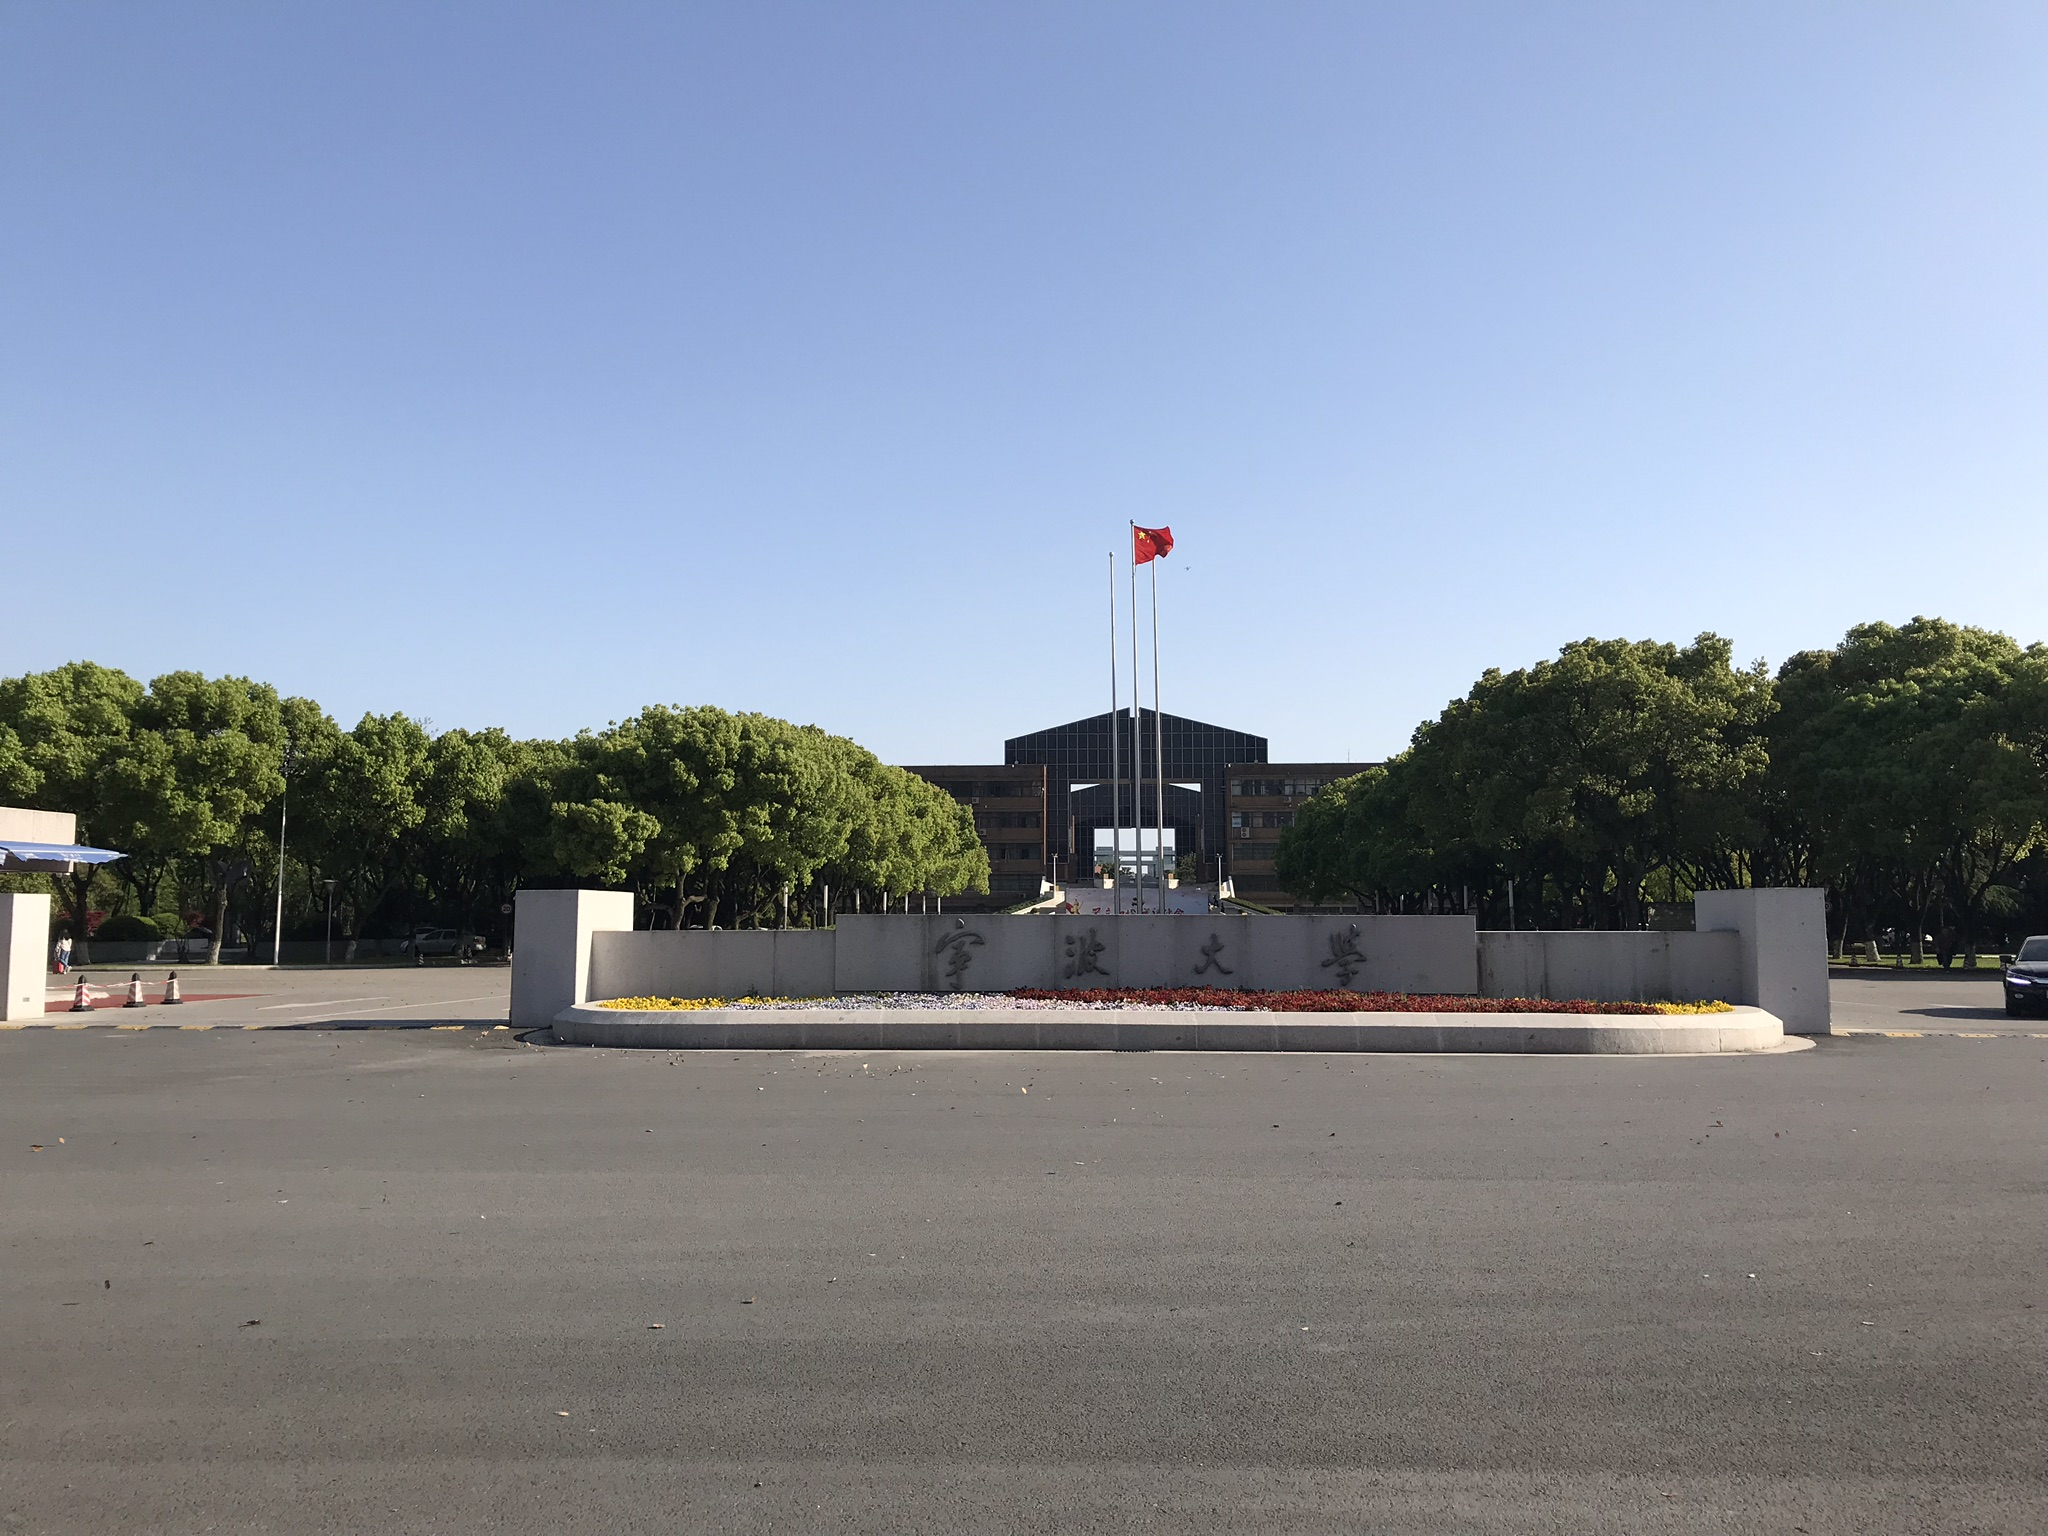
\includegraphics[width=0.82\textwidth]{figures/ningbo_university_gate.jpg}
  \caption{宁波大学正门示例图（图源：Nbfreeh，CC BY-SA 4.0，经 Wikimedia Commons）}
  \label{fig:ningbo-university-gate}
\end{figure}

\section{论文结构安排}
\label{sec:structure}

正文最多建议使用三级标题，即 \verb|\chapter|、\verb|\section| 和 \verb|\subsection|。目录默认显示到三级标题。若确有需要，可在本节中用列表概述各章职责，但不要手写章节编号。
